\RequirePackage{luatex85}
\documentclass[a4paper,class=article,border=0pt,crop,tikz]{standalone}
\usepackage{tikz}
\usepackage{pgf}
\usetikzlibrary{shapes.geometric}
\usepackage{color}
\definecolor{myviolet}{RGB}{55,54,112}
\usepackage{pgfplots}
\usepackage{siunitx}
\usetikzlibrary{calc,fadings,decorations.pathreplacing,decorations.pathmorphing,decorations.shapes,spy,arrows,arrows.meta,decorations.markings,fadings}
\usepackage{ifthen}
\pgfplotsset{compat=1.14}
% \usepgfplotslibrary{external}
% \tikzexternalize
\definecolor{violet}{RGB}{55,54,112}
\definecolor{darkgreen}{RGB}{75,141,75}
\definecolor{red}{RGB}{255,41,0}

\definecolor{green}{rgb}{0,0.6,0}
\definecolor{gray}{rgb}{0.5,0.5,0.5}
\definecolor{mauve}{rgb}{0.58,0,0.82}
\definecolor{blue}{rgb}{0.27,0.5,0.8}
\tikzset{
  double arrow/.style args={#1 colored by #2 and #3}{
    ->, >=latex, line width=#1,#2, % first arrow
    postaction={draw,->, >=latex, #3,line width=(#1)/2,
                shorten <=(#1)/4,shorten >=(#1)}, % second arrow
  }
}
%dimensions in decimeters

\begin{document}

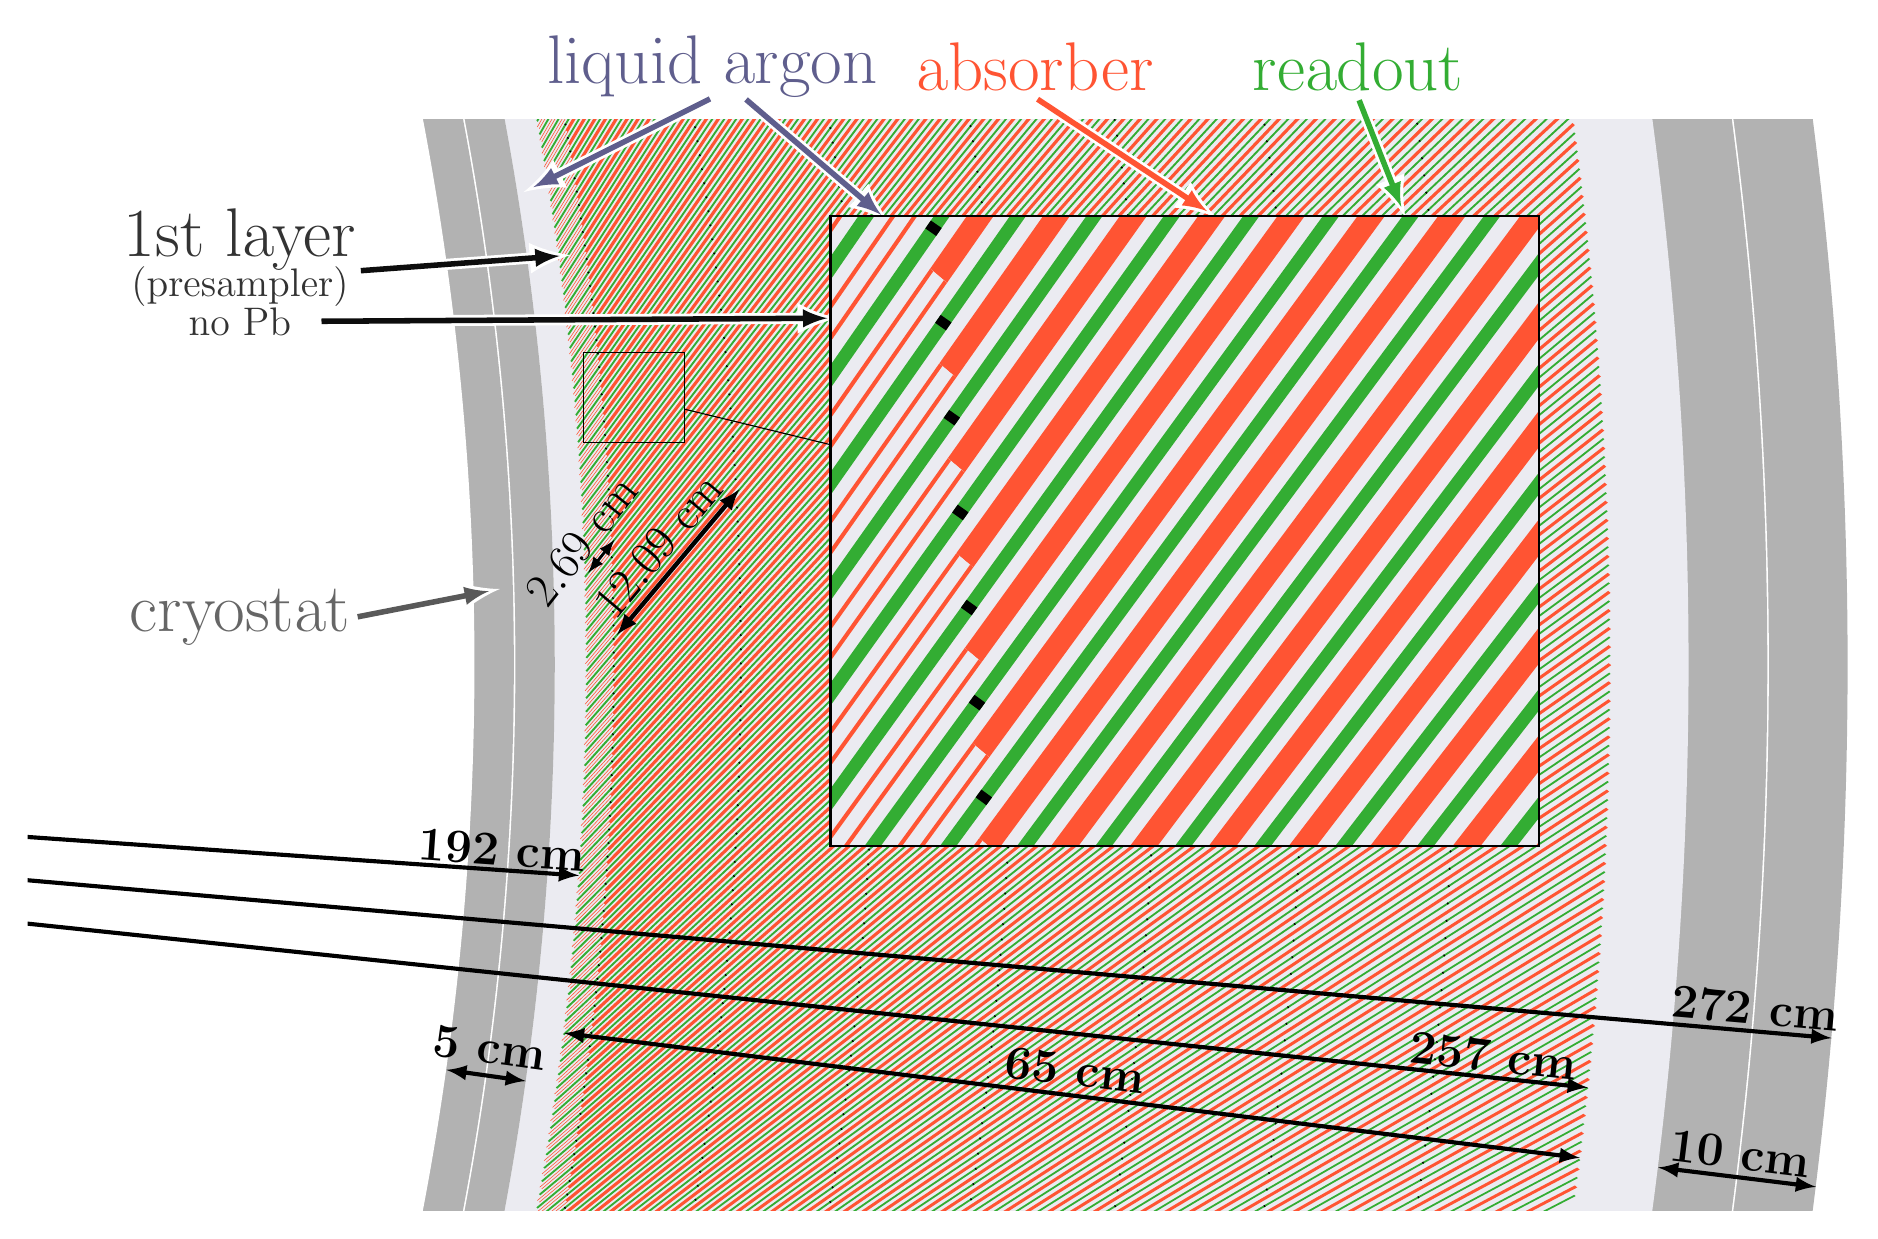
\begin{tikzpicture}[xscale=2,yscale=2,spy using outlines={rectangle, magnification=7, size=9cm, height = 8cm, connect spies}]\footnotesize
  \spy [ultra thick, black] on (39.,3.4) in node [fill=white] at (23,0.85);
  % \spy [ultra thick, black] on (39.45,3.4) in node [fill=white] at (25.5,1.5);
  \pgfmathsetmacro{\rin}{18.2}
  \pgfmathsetmacro{\rout}{27.5}
  \pgfmathsetmacro{\air}{0.3}
  \pgfmathsetmacro{\vacuum}{0.01}
  \pgfmathsetmacro{\calofront}{0.5}
  \pgfmathsetmacro{\caloback}{1}
  \pgfmathsetmacro{\halfcalofront}{{\calofront/2}}
  \pgfmathsetmacro{\halfcaloback}{{\caloback/2}}
  \pgfmathsetmacro{\bathfront}{0.2}
  \pgfmathsetmacro{\bathback}{0.5}
  \pgfmathsetmacro{\angle}{50}
  \pgfmathsetmacro{\absorber}{0.02}
  \pgfmathsetmacro{\readout}{0.012}
  \pgfmathsetmacro{\cell}{0.5}
  \pgfmathsetmacro{\tower}{0.75}
  \pgfmathsetmacro{\numplanes}{1408}
  \pgfmathsetmacro{\dphi}{360./\numplanes}
  \pgfmathsetmacro{\detin}{{\rin+\air+\calofront+\bathfront}}
  \pgfmathsetmacro{\detout}{{\rout-\air-\caloback-\bathback}}
  \pgfmathsetmacro{\plane}{sqrt(pow(\detout,2)-pow(\detin*sin(\angle) ,2))-\detin*cos(\angle)}
  \pgfmathsetmacro{\r}{{\detin+\plane/2}}
  \pgfmathsetmacro{\planeFirst}{{\plane/130*4}}
  \pgfmathsetmacro{\planeRest}{{\plane/130*18}}
  \pgfmathsetmacro{\phibins}{{int(\numplanes/2)}}
  \pgfmathsetmacro{\dPhiTower}{{360/\phibins}}
  \pgfmathsetmacro{\phiShow}{360/8}
  \pgfmathsetmacro{\phiOffsetFromY}{90-\phiShow/2}
  \pgfmathsetmacro{\phiOffsetFromX}{{\phiOffsetFromY-90}}
  \pgfmathsetmacro{\phiTowerHighlightOne}{-3}
  \pgfmathsetmacro{\highlitedTowerMinOne}{{(\phiTowerHighlightOne-0.5)*360/\phibins}}
  \pgfmathsetmacro{\highlitedTowerMaxOne}{{(\phiTowerHighlightOne+0.5)*360/\phibins}}
  \pgfmathsetmacro{\phiTowerHighlightTwo}{12}
  \pgfmathsetmacro{\highlitedTowerMinTwo}{{(\phiTowerHighlightTwo-0.5)*360/\phibins}}
  \pgfmathsetmacro{\highlitedTowerMaxTwo}{{(\phiTowerHighlightTwo+0.5)*360/\phibins}}
  \pgfmathsetmacro{\phiTowerHighlightThree}{3}
  \pgfmathsetmacro{\highlitedTowerMinThree}{{(\phiTowerHighlightThree-0.5)*360/\phibins}}
  \pgfmathsetmacro{\highlitedTowerMaxThree}{{(\phiTowerHighlightThree+0.5)*360/\phibins}}
  \pgfmathsetmacro{\shownumplanes}{int(\numplanes/(360/\phiShow))}
  \pgfmathsetmacro{\showphibins}{int(\phibins/(360/\phiShow))}
  \ifthenelse{\angle=50 \and \numplanes=1408}
  { \pgfmathsetmacro{\ione}{{81.5}}
    \pgfmathsetmacro{\itwo}{{88.5}}
  }{\ifthenelse{\angle=30 \and \numplanes=1408}
    { \pgfmathsetmacro{\ione}{{81.5}}
      \pgfmathsetmacro{\itwo}{{84.5}}
    }{\ifthenelse{\angle=0 \and \numplanes=1408}
      { \pgfmathsetmacro{\ione}{{80.5}}
        \pgfmathsetmacro{\itwo}{{78.5}}
      }{\ifthenelse{\angle=50 \and \numplanes=1280}
        { \pgfmathsetmacro{\ione}{{73.5}}
          \pgfmathsetmacro{\itwo}{{79.5}}
        }{\ifthenelse{\angle=30 \and \numplanes=1280}
          { \pgfmathsetmacro{\ione}{{73.5}}
            \pgfmathsetmacro{\itwo}{{76.5}}
          }{\ifthenelse{\angle=0 \and \numplanes=1280}
            { \pgfmathsetmacro{\ione}{{72.5}}
              \pgfmathsetmacro{\itwo}{{70.5}}
            }{
            }
          }
        }
      }
    }
  }

  \clip ({0.86*\rin},{-\rin/5.25}) rectangle ({0.99*\rout}, {\rin/4.5});
  %\clip ({1.05*\rin},{-\rin/10}) rectangle ({1.3*\rin}, {\rin/10});

  % CRYOSTAT
  \begin{scope}[black!30]
    \fill (0,0)  ++(\phiOffsetFromX:{\rout-\air+\vacuum}) arc (\phiOffsetFromX:{\phiOffsetFromX+\phiShow}:{\rout-\air+\vacuum});
    \fill[fill=white] (0,0) ++(\phiOffsetFromX:{\rout-\air+\vacuum-\halfcaloback})  arc (\phiOffsetFromX:{\phiOffsetFromX+\phiShow}:{\rout-\air+\vacuum-\halfcaloback});
    \fill (0,0) ++ (\phiOffsetFromX:{\rout-\air-\halfcaloback}) arc (\phiOffsetFromX:{\phiOffsetFromX+\phiShow}:{\rout-\air-\halfcaloback});
    \fill[fill=violet!10] (0,0) ++(\phiOffsetFromX:{\rout-\air-\caloback}) arc (\phiOffsetFromX:{\phiOffsetFromX+\phiShow}:{\rout-\air-\caloback})
    -- ({\phiOffsetFromX+\phiShow}:{\rin+\air+\calofront}) arc ({\phiOffsetFromX+\phiShow}:\phiOffsetFromX:{\rin+\air+\calofront}) -- (\phiOffsetFromX:{\rout-\air-\caloback});
    \fill (0,0) ++(\phiOffsetFromX:{\rin+\air+\calofront}) arc (\phiOffsetFromX:{\phiOffsetFromX+\phiShow}:{\rin+\air+\calofront});
    \fill[fill=white] (0,0) ++ (\phiOffsetFromX:{\rin+\air+\halfcalofront}) arc (\phiOffsetFromX:{\phiOffsetFromX+\phiShow}:{\rin+\air+\halfcalofront});
    \fill (0,0) ++(\phiOffsetFromX:{\rin+\air-\vacuum+\halfcalofront}) arc (\phiOffsetFromX:{\phiOffsetFromX+\phiShow}:{\rin+\air-\vacuum+\halfcalofront});
    \fill[fill=white] (0,0) ++(\phiOffsetFromX:{\rin+\air-\vacuum}) arc (\phiOffsetFromX:{\phiOffsetFromX+\phiShow}:{\rin+\air-\vacuum});
  \end{scope}

  % ABSORBER - only outer in the first layer
  \begin{scope}[red!80, line width = 0.005]
    \foreach \i in {0,..., \shownumplanes}
    {
      \pgfmathsetmacro{\phi}{{\phiOffsetFromY+\i*\dphi}}
      % centre of radial
      \pgfmathsetmacro{\xB}{{(\detin+\plane/2)*sin(\phi)}}
      \pgfmathsetmacro{\yB}{{(\detin+\plane/2)*cos(\phi)}}
      % position of begining of a plane
      \pgfmathsetmacro{\xA}{{\detin*sin(\phi)}}
      \pgfmathsetmacro{\yA}{{\detin*cos(\phi)}}
      % rotated plane
      \pgfmathsetmacro{\xC}{{\xA+2*(\xB-\xA)*cos(\angle)-2*(\yB-\yA)*sin(\angle)}}
      \pgfmathsetmacro{\yC}{{\yA+2*(\xB-\xA)*sin(\angle)+2*(\yB-\yA)*cos(\angle)}}
      % new begining of a plane
      \pgfmathsetmacro{\xA}{{\xA+\planeFirst*sin(\phi)*cos(\angle)-\planeFirst*cos(\phi)*sin(\angle)}}
      \pgfmathsetmacro{\yA}{{\yA+\planeFirst*sin(\phi)*sin(\angle)+\planeFirst*cos(\phi)*cos(\angle)}}
      % rectangle halfwidth
      \pgfmathsetmacro{\xShift}{{(\absorber/2)*sin(\angle)}}
      \pgfmathsetmacro{\yShift}{{(\absorber/2)*cos(\angle)}}

      \fill ({\xA-\xShift}, {\yA+\yShift}) -- ({\xA+\xShift}, {\yA-\yShift})
      -- ({\xC+\xShift}, {\yC-\yShift})    -- ({\xC-\xShift}, {\yC+\yShift})
      -- ({\xA-\xShift}, {\yA+\yShift}) ;
    }
  \end{scope}
  % ABSORBER - not in the first layer
  \begin{scope}[red!80, line width = 0.005]
    \foreach \i in {0,..., \shownumplanes}
    {
      \pgfmathsetmacro{\phi}{{\phiOffsetFromY+\i*\dphi}}
      % centre of radial
      \pgfmathsetmacro{\xB}{{(\detin+\planeFirst/2)*sin(\phi)}}
      \pgfmathsetmacro{\yB}{{(\detin+\planeFirst/2)*cos(\phi)}}
      % position of begining of a plane
      \pgfmathsetmacro{\xA}{{\detin*sin(\phi)}}
      \pgfmathsetmacro{\yA}{{\detin*cos(\phi)}}
      % rotated plane
      \pgfmathsetmacro{\xC}{{\xA+2*(\xB-\xA)*cos(\angle)-2*(\yB-\yA)*sin(\angle)}}
      \pgfmathsetmacro{\yC}{{\yA+2*(\xB-\xA)*sin(\angle)+2*(\yB-\yA)*cos(\angle)}}
      % rectangle halfwidth
      \pgfmathsetmacro{\xShift}{{(\absorber/2)*sin(\angle)}}
      \pgfmathsetmacro{\yShift}{{(\absorber/2)*cos(\angle)}}
      \pgfmathsetmacro{\xShiftThin}{{(\absorber/5.4)*sin(\angle)}}
      \pgfmathsetmacro{\yShiftThin}{{(\absorber/5.4)*cos(\angle)}}

      \fill[violet!10] ({\xA-\xShift}, {\yA+\yShift}) -- ({\xA+\xShift}, {\yA-\yShift})
      -- ({\xC+\xShift}, {\yC-\yShift})    -- ({\xC-\xShift}, {\yC+\yShift})
      -- ({\xA-\xShift}, {\yA+\yShift}) ;

      \fill ({\xA-\xShift}, {\yA+\yShift}) % pocz lewa
      -- ({\xA-\xShift+\xShiftThin}, {\yA+\yShift-\yShiftThin}) % pocz prawa
      -- ({\xC-\xShift+\xShiftThin}, {\yC+\yShift-\yShiftThin}) % kon prawa
      -- ({\xC-\xShift}, {\yC+\yShift}) % kon lewa
      -- ({\xA-\xShift}, {\yA+\yShift}) ; % back

      \fill ({\xA+\xShift-\xShiftThin}, {\yA-\yShift+\yShiftThin}) % pocz lewa
      -- ({\xA+\xShift}, {\yA-\yShift}) % pocz prawa
      -- ({\xC+\xShift}, {\yC-\yShift}) % kon prawa
      -- ({\xC+\xShift-\xShiftThin}, {\yC-\yShift+\yShiftThin}) % kon lewa
      -- ({\xA+\xShift-\xShiftThin}, {\yA-\yShift+\yShiftThin}) ; % back
    }
  \end{scope}
  % READOUT
  \begin{scope}[green!80, line width = 0.005]
    \foreach \i in {0,..., \shownumplanes}
    {
      \pgfmathsetmacro{\phi}{{\phiOffsetFromY+(0.5+\i)*\dphi}}
      % centre of radial
      \pgfmathsetmacro{\xB}{{(\detin+\plane/2)*sin(\phi)}}
      \pgfmathsetmacro{\yB}{{(\detin+\plane/2)*cos(\phi)}}
      % position of begining of a plane
      \pgfmathsetmacro{\xA}{{\detin*sin(\phi)}}
      \pgfmathsetmacro{\yA}{{\detin*cos(\phi)}}
      % rotated plane
      \pgfmathsetmacro{\xC}{{\xA+2*(\xB-\xA)*cos(\angle)-2*(\yB-\yA)*sin(\angle)}}
      \pgfmathsetmacro{\yC}{{\yA+2*(\xB-\xA)*sin(\angle)+2*(\yB-\yA)*cos(\angle)}}
      % rectangle halfwidth
      \pgfmathsetmacro{\xShift}{{(\readout/2)*sin(\angle)}}
      \pgfmathsetmacro{\yShift}{{(\readout/2)*cos(\angle)}}

      \fill ({\xA-\xShift}, {\yA+\yShift}) -- ({\xA+\xShift}, {\yA-\yShift})
      -- ({\xC+\xShift}, {\yC-\yShift})    -- ({\xC-\xShift}, {\yC+\yShift})
      -- ({\xA-\xShift}, {\yA+\yShift}) ;
    }
  \end{scope}

  % CELLS: longitudinal borders
  \begin{scope}[black, line width = {\cell}]
    \foreach \i in {0,..., \shownumplanes}
    {
      \pgfmathsetmacro{\phiReadout}{{\phiOffsetFromY+(\i+0.5)*\dphi}}
      % centre of unrotated plane
      \pgfmathsetmacro{\xBFirst}{{(\detin)*sin(\phiReadout)}} % beginning of detector
      \pgfmathsetmacro{\yBFirst}{{(\detin)*cos(\phiReadout)}}
      \pgfmathsetmacro{\xBnext}{{(\detin+\planeFirst)*sin(\phiReadout)}} % end of first layer
      \pgfmathsetmacro{\yBnext}{{(\detin+\planeFirst)*cos(\phiReadout)}}
      % begin of plane
      \pgfmathsetmacro{\xAFirst}{{\detin*sin(\phiReadout)}}
      \pgfmathsetmacro{\yAFirst}{{\detin*cos(\phiReadout)}}
      % rotated plane
      \pgfmathsetmacro{\xCFirst}{{\xAFirst+(\xBFirst-\xAFirst)*cos(\angle)-(\yBFirst-\yAFirst)*sin(\angle)}}
      \pgfmathsetmacro{\yCFirst}{{\yAFirst+(\xBFirst-\xAFirst)*sin(\angle)+(\yBFirst-\yAFirst)*cos(\angle)}}
      \pgfmathsetmacro{\xCnext}{{\xAFirst+(\xBnext-\xAFirst)*cos(\angle)-(\yBnext-\yAFirst)*sin(\angle)}}
      \pgfmathsetmacro{\yCnext}{{\yAFirst+(\xBnext-\xAFirst)*sin(\angle)+(\yBnext-\yAFirst)*cos(\angle)}}

      \pgfmathsetmacro{\cellInThickness}{{\readout/2}};
      \pgfmathsetmacro{\cellOutThickness}{{\readout/2}};

      \pgfmathsetmacro{\phiCentre}{{atan((\yCFirst+\yCnext)/(\xCFirst+\xCnext))}};
      \foreach \j in {0,..., 6}
      {
        \pgfmathsetmacro{\xB}{{(\detin+\planeFirst+\j*\planeRest)*sin(\phiReadout)}};
        \pgfmathsetmacro{\yB}{{(\detin+\planeFirst+\j*\planeRest)*cos(\phiReadout)}};
        \pgfmathsetmacro{\xBnext}{{(\detin+\planeFirst+(\j+1)*\planeRest)*sin(\phiReadout)}};
        \pgfmathsetmacro{\yBnext}{{(\detin+\planeFirst+(\j+1)*\planeRest)*cos(\phiReadout)}};
        \pgfmathsetmacro{\xA}{{\detin*sin(\phiReadout)}};
        \pgfmathsetmacro{\yA}{{\detin*cos(\phiReadout)}};
        \pgfmathsetmacro{\xC}{{\xA+(\xB-\xA)*cos(\angle)-(\yB-\yA)*sin(\angle)}};
        \pgfmathsetmacro{\yC}{{\yA+(\xB-\xA)*sin(\angle)+(\yB-\yA)*cos(\angle)}};
        \pgfmathsetmacro{\xCnext}{{\xA+(\xBnext-\xA)*cos(\angle)-(\yBnext-\yA)*sin(\angle)}};
        \pgfmathsetmacro{\yCnext}{{\yA+(\xBnext-\xA)*sin(\angle)+(\yBnext-\yA)*cos(\angle)}};

        \pgfmathsetmacro{\phiCentre}{{atan((\yC+\yCnext)/2/((\xC+\xCnext)/2))}}
              \draw ({\xC - (\cellOutThickness)*cos(-\angle+\phiReadout)}, {\yC + (\cellOutThickness)*sin(-\angle+\phiReadout)})
              -- ({\xC + (\cellOutThickness)*cos(-\angle+\phiReadout)}, {\yC - (\cellOutThickness)*sin(-\angle+\phiReadout)});
      }
    }
  \end{scope}

  % % tower
  % \begin{scope}[black, line width = \tower]
  %   \foreach \i in {0,..., \showphibins}
  %   {
  %     \pgfmathsetmacro{\phiTower}{{\phiOffsetFromX+(\i+0.5)*\dPhiTower}}
  %     \draw ({\phiTower}:\detin) -- ({\phiTower}: \detout);
  %   }
  % \end{scope}

  % \begin{scope}[black!20]
  %   \draw[dashed] (0,0) ++ (30:{\rin}) arc (30:-30:{\rin});
  %   \draw[dashed] (0,0) ++ (30:{\rout}) arc (30:-30:{\rout});
  % \end{scope}
  \fill[white] ({0.85*\rin},{\rin/5.25}) rectangle ({1.1*\rout}, {\rin/3});

  \begin{scope}[black, line width = {\tower*2}]
    \pgfmathsetmacro{\dPhiTowerRadians}{{6.28/\phibins}};
    \pgfmathsetmacro{\phiCluster}{{\phiTowerHighlightTwo-\phiTowerHighlightOne}};
    \pgfmathsetmacro{\dPhiClusterRadians}{{6.28/\phibins*\phiCluster}};
    % \pgfmathsetmacro{\phitextOne}{90+\highlitedTowerMinOne*\dphi};
    % \message{\phitextOne};
    % \draw[<->,line width = {\tower}, >=latex, bend right] ({\highlitedTowerMinOne}:{\detout+0.1}) -- ({\highlitedTowerMaxOne}:{\detout+0.1}) node [below, midway,,rotate=\phitextOne] {\Large $\frac{2\pi}{\phibins}$};
    % \pgfmathsetmacro{\phitextThree}{90+\highlitedTowerMinThree*\dphi};
    % \draw[<->, >=latex, line width = {\tower},bend right] (\highlitedTowerMinThree:{\detout+0.1}) -- ({\highlitedTowerMaxThree}:{\detout+0.1}) node [below, midway,rotate=\phitextThree] {\large \num[round-mode=places,round-precision=4]{\dPhiTowerRadians} rad};
    % \pgfmathsetmacro{\phitextTwo}{90+\highlitedTowerMinTwo*\dphi};
    % \draw[<->, >=latex, line width = {\tower},bend right] ({\highlitedTowerMinTwo}:{\detout+0.1}) -- ({\highlitedTowerMaxTwo}:{\detout+0.1}) node [below, midway ,rotate=\phitextTwo] {\large {\dPhiTower}$^\circ$};
    % \pgfmathsetmacro{\phitextCluster}{{90+(\phiTowerHighlightTwo-\phiTowerHighlightOne)*\dphi}};
    % \draw[<->,line width = {\tower}, >=latex] (0,0) ++ ({\highlitedTowerMaxTwo}:{\detout+0.1}) arc ({\highlitedTowerMaxTwo}:{\highlitedTowerMinOne}:{\detout+0.1}) node [below, midway,rotate=\phitextCluster] {\large \num[round-mode=places,round-precision=0]{\phiCluster}$\Delta\varphi$ = \num[round-mode=places,round-precision=3]{\dPhiClusterRadians} rad};
    % \spy [blue] on (20,0{\rin},0) in node [fill=white] at (25,1.5);
%    \draw[->,>=latex] (-3:{\rin-5}) -- (-3:\rin+\air-\vacuum) node [at end, above, xshift=-1cm, rotate=-3] {\textbf{\LARGE 185 cm}};
    \draw[->,>=latex] (-5:{\rin-5}) -- (-5:\rout-\air+\vacuum) node [at end, above, xshift=-1cm, yshift=0.05cm, rotate=-5] {\textbf{\LARGE 272 cm}};
    \draw[->,>=latex] (-4:{\rin-5}) -- (-4:\detin) node [at end, above, xshift=-1cm, rotate=-4] {\textbf{\LARGE 192 cm}};
    \draw[->,>=latex] (-6:{\rin-5}) -- (-6:\detout) node [at end, xshift=-1.2cm, yshift=0.4cm, rotate=-6] {\textbf{\LARGE 257 cm}};
    \draw[<->,>=latex] (-7:\detin) -- (-7:\detout) node [above,midway,rotate=-7] {\textbf{\LARGE 65 cm}};
    % \draw[<->,>=latex] (-8:{\rin+\air-\vacuum}) -- (-8:\rin) node [above, near end, xshift=0.2cm, rotate=-8] {\large 3 cm};
    % \draw[<->,>=latex] (-6.:{\rout-\air+\vacuum}) -- (-6.:\rout) node [above, near end, xshift=-0.05cm, rotate=-6.] {\large 3 cm};
    \draw[<->,>=latex] (-8:{\rin+\air-\vacuum}) -- (-8:\rin+\air+\calofront) node [above, xshift=-0.5cm, yshift=0.1cm, rotate=-8] {\textbf{\LARGE 5 cm}};
    \draw[<->,>=latex] (-7:{\detout+\bathback}) -- (-7:\detout+\bathback+\caloback+\vacuum) node [above, xshift=-1cm, yshift=0.1cm, rotate=-7] {\textbf{\LARGE 10 cm}};
    %% \node (angLabel) at (6:{\rout-1}) {\Huge\bf {\numplanes} absorbers};
    %% \node (angLabel) at ({{0.86*\rin+(0.99*\rout-0.86*\rin)/2}},4.3) {\Huge\textbf{FCC-hh barrel ECAL}};
%%%%%    \node [below of = planeLabel] {\Huge{ $\Delta\varphi=$\num[round-mode=places,round-precision=4]{\dPhiTowerRadians}}};
    \node[red!80] at (22.05,3.8) {\Huge absorber};
    %% \draw[->, >=latex, red!80] (22.05,3.6) -- (23.2, 2.84);
    \draw[double arrow=4pt colored by white and red!80] (22.05,3.6) -- (23.2, 2.84);
    \node[green!80] at (24.1,3.8) {\Huge readout};
    %% \draw[->, >=latex, green!80] (24.1,3.6) -- (24.4, 2.84);
    \draw[double arrow=4pt colored by white and green!80] (24.1,3.6) -- (24.4, 2.84);
    \node[black!60] at (17.,0.3) {\Huge cryostat};
    %% \draw[->, >=latex, black!65] (17.73,0.3) -- (18.65, 0.48);
    \draw[double arrow=4pt colored by white and black!65] (17.73,0.3) -- (18.65, 0.48);
    \node[violet!80] at (20.,3.8) {\Huge liquid argon };
    %% \node[violet!80] at (17.,1.1) {\Huge argon};
    %% \draw[->, >=latex, violet!80] (20,3.6) -- (18.95, 3.);
    %% \draw[->, >=latex, violet!80] (20.2,3.6) -- (21, 2.84);
    \draw[double arrow=4pt colored by white and violet!80] (20,3.6) -- (18.8, 3.);
    \draw[double arrow=4pt colored by white and violet!80] (20.2,3.6) -- (21.125, 2.81);
    \node[black!80] at (17,2.7) {\Huge 1st layer};
    \node[black!80] at (17,2.4) {\Large (presampler)};
    \node[black!80] at (17,2.18) {\Large no Pb};
    %% \draw[->, >=latex, black!95] (18.,2.6) -- (19.1, 2.28);
    \draw[double arrow=4pt colored by white and black!95] (17.75,2.5) -- (19.1, 2.6);
    \draw[double arrow=4pt colored by white and black!95] (17.5,2.18) -- (20.8, 2.2);
  \end{scope}


  % CELLS: longitudinal borders
  \begin{scope}[violet!80, line width = \cell]
    \foreach \i in {0,..., \shownumplanes}
    {
      \pgfmathsetmacro{\phiReadout}{{\phiOffsetFromY+(\i)*\dphi}}
      % centre of unrotated plane
      \pgfmathsetmacro{\xBFirst}{{(\detin)*sin(\phiReadout)}} % beginning of detector
      \pgfmathsetmacro{\yBFirst}{{(\detin)*cos(\phiReadout)}}
      \pgfmathsetmacro{\xBnext}{{(\detin+\planeFirst)*sin(\phiReadout)}} % end of first layer
      \pgfmathsetmacro{\yBnext}{{(\detin+\planeFirst)*cos(\phiReadout)}}
      % begin of plane
      \pgfmathsetmacro{\xAFirst}{{\detin*sin(\phiReadout)}}
      \pgfmathsetmacro{\yAFirst}{{\detin*cos(\phiReadout)}}
      % rotated plane
      \pgfmathsetmacro{\xCFirst}{{\xAFirst+(\xBFirst-\xAFirst)*cos(\angle)-(\yBFirst-\yAFirst)*sin(\angle)}}
      \pgfmathsetmacro{\yCFirst}{{\yAFirst+(\xBFirst-\xAFirst)*sin(\angle)+(\yBFirst-\yAFirst)*cos(\angle)}}
      \pgfmathsetmacro{\xCnext}{{\xAFirst+(\xBnext-\xAFirst)*cos(\angle)-(\yBnext-\yAFirst)*sin(\angle)}}
      \pgfmathsetmacro{\yCnext}{{\yAFirst+(\xBnext-\xAFirst)*sin(\angle)+(\yBnext-\yAFirst)*cos(\angle)}}
      \pgfmathsetmacro{\activeInThickness}{{\detin*sin(\dphi/2.)*cos(\angle)}};
      \pgfmathsetmacro{\activeOutThickness}{{\detin+\plane)*sin(\dphi/2.)*cos(\angle)}};
      \pgfmathsetmacro{\xIntersect}{{(\detin*(tan(\angle)-cos(\dphi/2)*tan(\angle+\dphi/2))-\plane*sin(\dphi/2))/(tan(\angle)-tan(\angle+\dphi/2))}};
      \pgfmathsetmacro{\yIntersect}{{tan(\angle)*\xIntersect+\detin*(sin(\dphi/2)-tan(\angle))+\plane*sin(\dphi/2)}};
      \pgfmathsetmacro{\correction}{{\plane-sqrt(pow(\xIntersect-\detin*cos(\dphi/2),2)+pow(\yIntersect-\detin*sin(\dphi/2),2))}};
      \pgfmathsetmacro{\activeOutThickness}{{\activeOutThickness+2*\correction*sin(\dphi/4.)}};
      \pgfmathsetmacro{\cellIncrease}{{(\activeOutThickness-\activeInThickness) / 130}};
      \pgfmathsetmacro{\cellInThickness}{{\activeInThickness}};
      \pgfmathsetmacro{\cellOutThickness}{{\activeInThickness + \cellIncrease * 4}};

      \pgfmathsetmacro{\phiCentre}{{atan((\yCFirst+\yCnext)/(\xCFirst+\xCnext))}}

      \ifthenelse{\i=\ione}
      {
        \message{\planeFirst};
        \pgfmathsetmacro{\planeFirstInCm}{{10.*\planeFirst}};
        % \fill[%decorate, decoration={random steps,segment length=0.2mm, amplitude=0.01mm},
        % thick, rounded corners=1ex,,white,fill opacity=0.7]  ({\xCFirst}, {\yCFirst})  circle ({\planeFirst});
        \draw[<->,>=latex,black,line width=1pt] ({\xCFirst + \cellInThickness*cos(-\angle+\phiReadout)}, {\yCFirst - \cellInThickness*sin(-\angle+\phiReadout)}) -- ({\xCnext + \cellOutThickness*cos(-\angle+\phiReadout)}, {\yCnext - \cellOutThickness*sin(-\angle+\phiReadout)}) node [above, midway, rotate={90+\angle-\phiReadout}] {\LARGE \num[round-mode=places,round-precision=2]{\planeFirstInCm} cm};
      } {}

      \foreach \j in {0,..., 6}
      {
        \pgfmathsetmacro{\xB}{{(\detin+\planeFirst+\j*\planeRest)*sin(\phiReadout)}};
        \pgfmathsetmacro{\yB}{{(\detin+\planeFirst+\j*\planeRest)*cos(\phiReadout)}};
        \pgfmathsetmacro{\xBnext}{{(\detin+\planeFirst+(\j+1)*\planeRest)*sin(\phiReadout)}};
        \pgfmathsetmacro{\yBnext}{{(\detin+\planeFirst+(\j+1)*\planeRest)*cos(\phiReadout)}};
        \pgfmathsetmacro{\xA}{{\detin*sin(\phiReadout)}};
        \pgfmathsetmacro{\yA}{{\detin*cos(\phiReadout)}};
        \pgfmathsetmacro{\xC}{{\xA+(\xB-\xA)*cos(\angle)-(\yB-\yA)*sin(\angle)}};
        \pgfmathsetmacro{\yC}{{\yA+(\xB-\xA)*sin(\angle)+(\yB-\yA)*cos(\angle)}};
        \pgfmathsetmacro{\xCnext}{{\xA+(\xBnext-\xA)*cos(\angle)-(\yBnext-\yA)*sin(\angle)}};
        \pgfmathsetmacro{\yCnext}{{\yA+(\xBnext-\xA)*sin(\angle)+(\yBnext-\yA)*cos(\angle)}};

        \pgfmathsetmacro{\phiCentre}{{atan((\yC+\yCnext)/2/((\xC+\xCnext)/2))}}
        \ifthenelse{\i=\itwo \and \j=0}
        {
          \message{\planeRest};
          \pgfmathsetmacro{\planeRestInCm}{{10.*\planeRest}};
          % \fill[%decorate, decoration={random steps,segment length=0.2mm, amplitude=0.01mm},
          % thick, rounded corners=1ex,,white, opacity=0.6]  ({\xC}, {\yC}) circle ({\planeRest});
          \draw[<->,>=latex, ultra thick,black]({\xC + \cellInThickness*cos(-\angle+\phiReadout)}, {\yC - \cellInThickness*sin(-\angle+\phiReadout)}) -- ({\xCnext + \cellOutThickness*cos(-\angle+\phiReadout)}, {\yCnext - \cellOutThickness*sin(-\angle+\phiReadout)}) node [above, midway, rotate={90+\angle-\phiReadout}] {\LARGE \num[round-mode=places,round-precision=2]{\planeRestInCm} cm};
        } {}
      }
    }
  \end{scope}

  % \draw[step=0.1,black,thin] (0,0) grid (20,20);
  % \draw[step=1,black] (0,0) grid (20,20);
\end{tikzpicture}
\end{document}
